\subsection{Previous courses page (Vlad)}

This page offers an overview for the courses the student took combined by semester. The semester can be changed via a navbar on top and the list of courses changes.\\\\
All the courses are presented in a table each row being separated by a new line for better understanding of the page. Each course has a default picture so the user can easily find the desired course in the list. \\
Each course has as information the final grade which was obtained by the student and a check mark if it was a passing grade. If the grade is below 45\% the sign changes to a red cross. This can be seen for GenCS where the grade is 35\%.\\
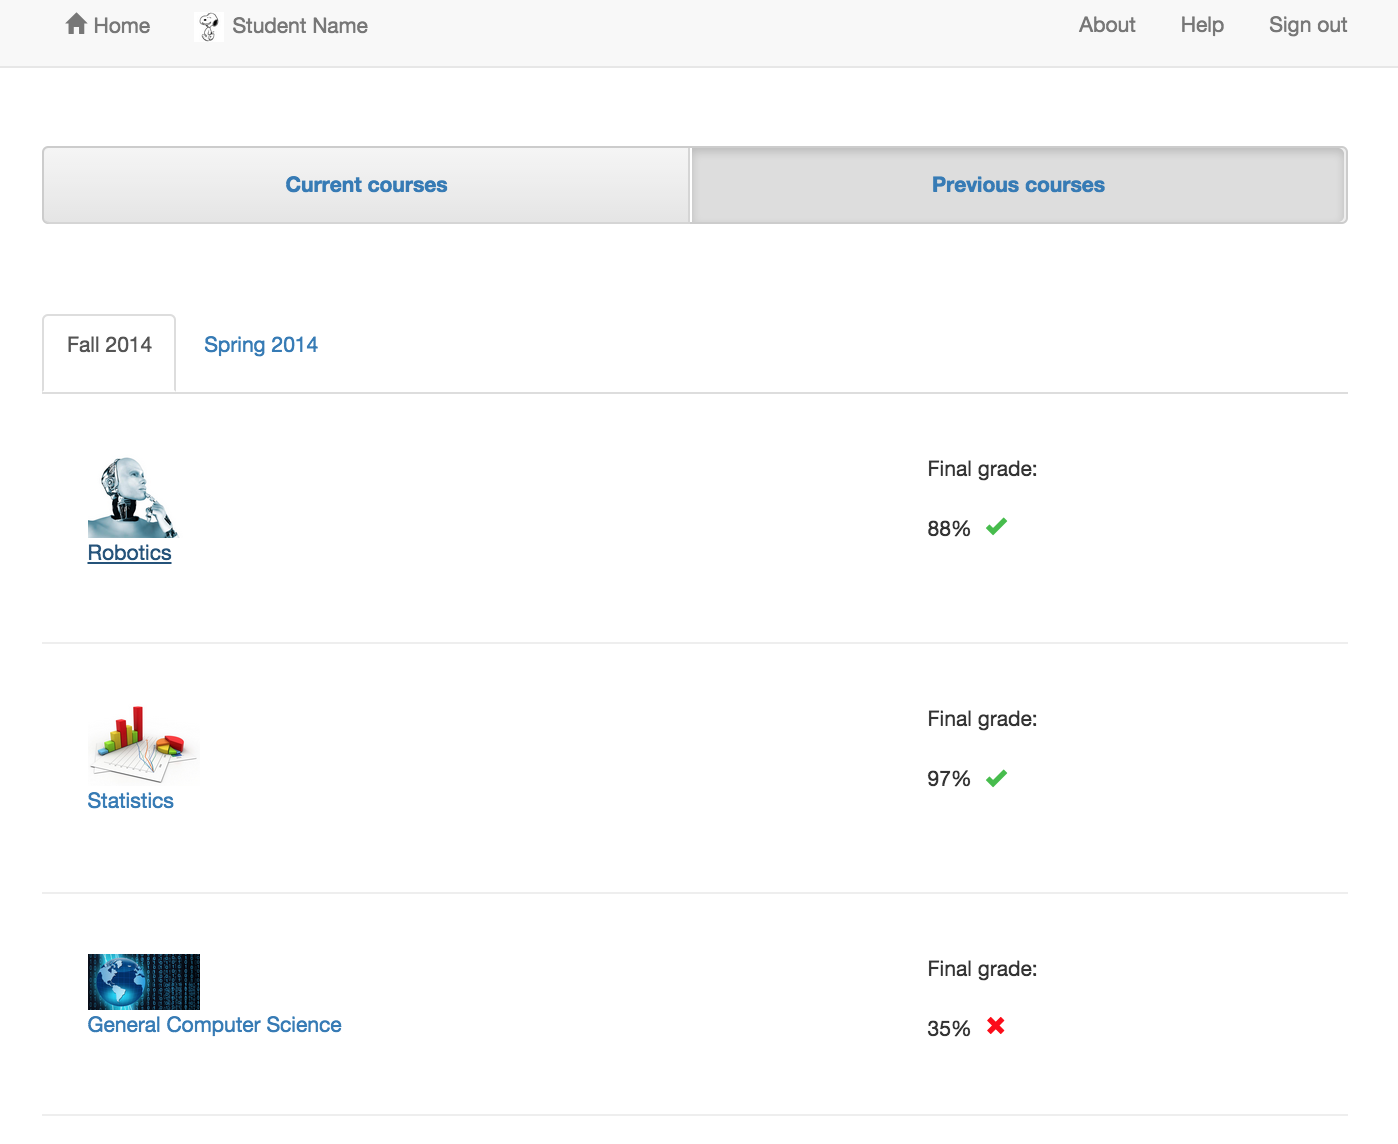
\includegraphics[width=.85\textwidth]{screenshots/PrevoiusCoursesOverview.png}

After the student clicks on a course (either picture or link this page is presented).\\

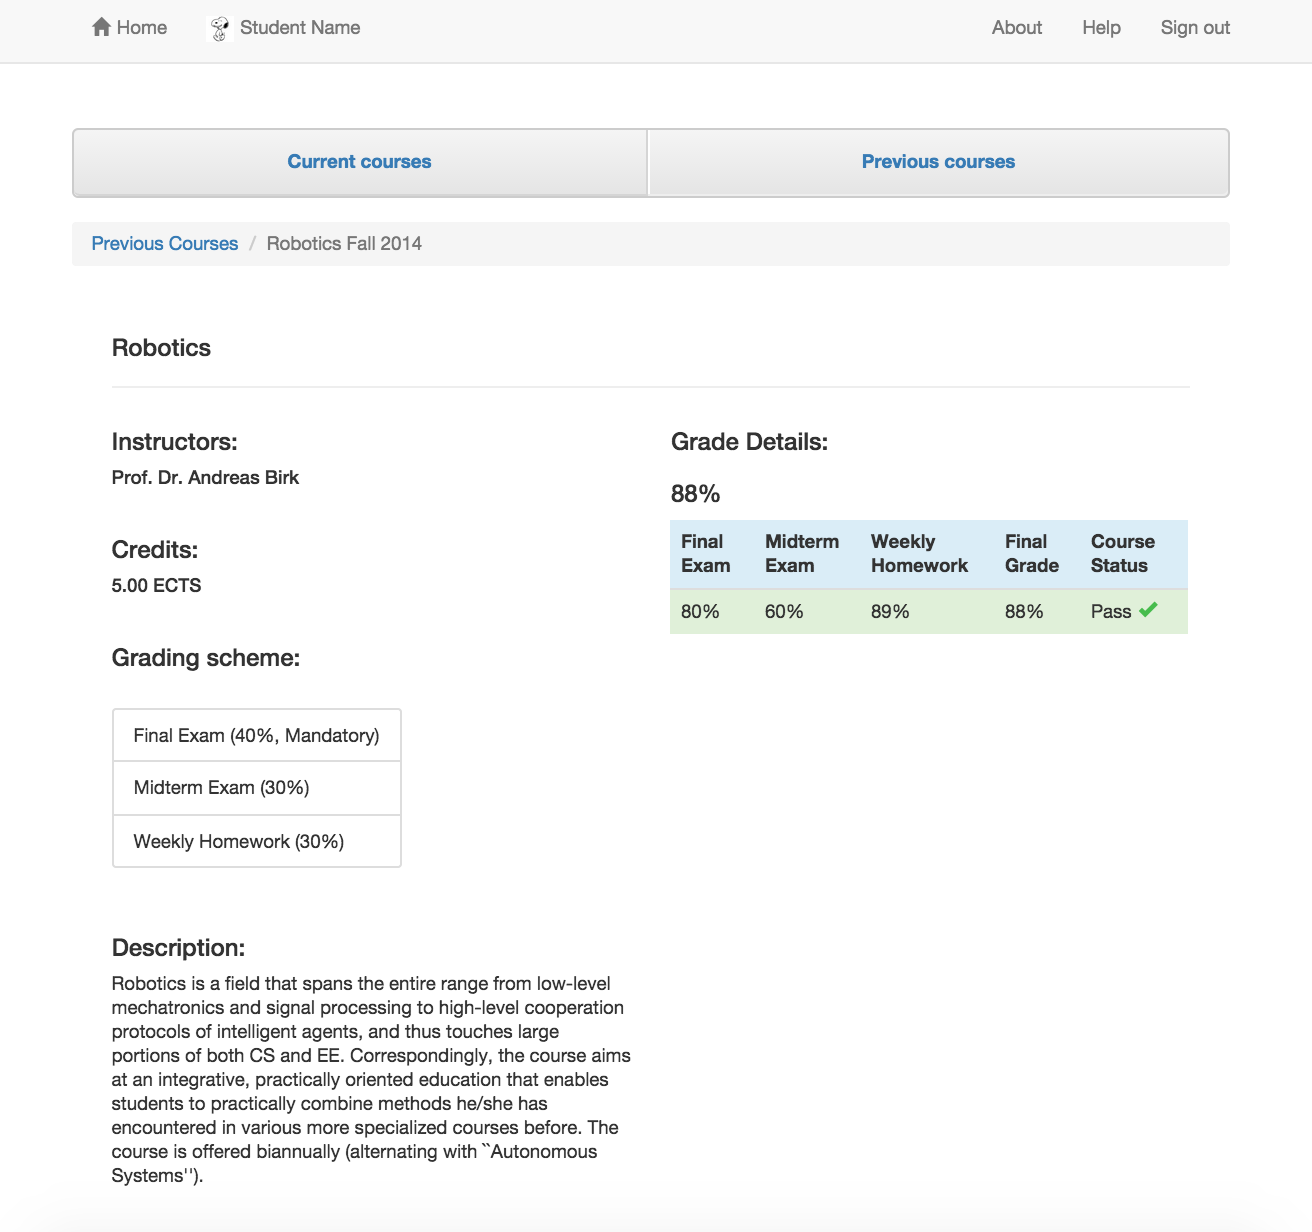
\includegraphics[width=.85\textwidth]{screenshots/PreviousCourseDetail.png}

The student can see the instructor, how may credits he got for the course, grading scheme and the description. We show in a table the grade components and the score he got for each of them. We use green as background for passes course and red for a course which has been failed.
=======
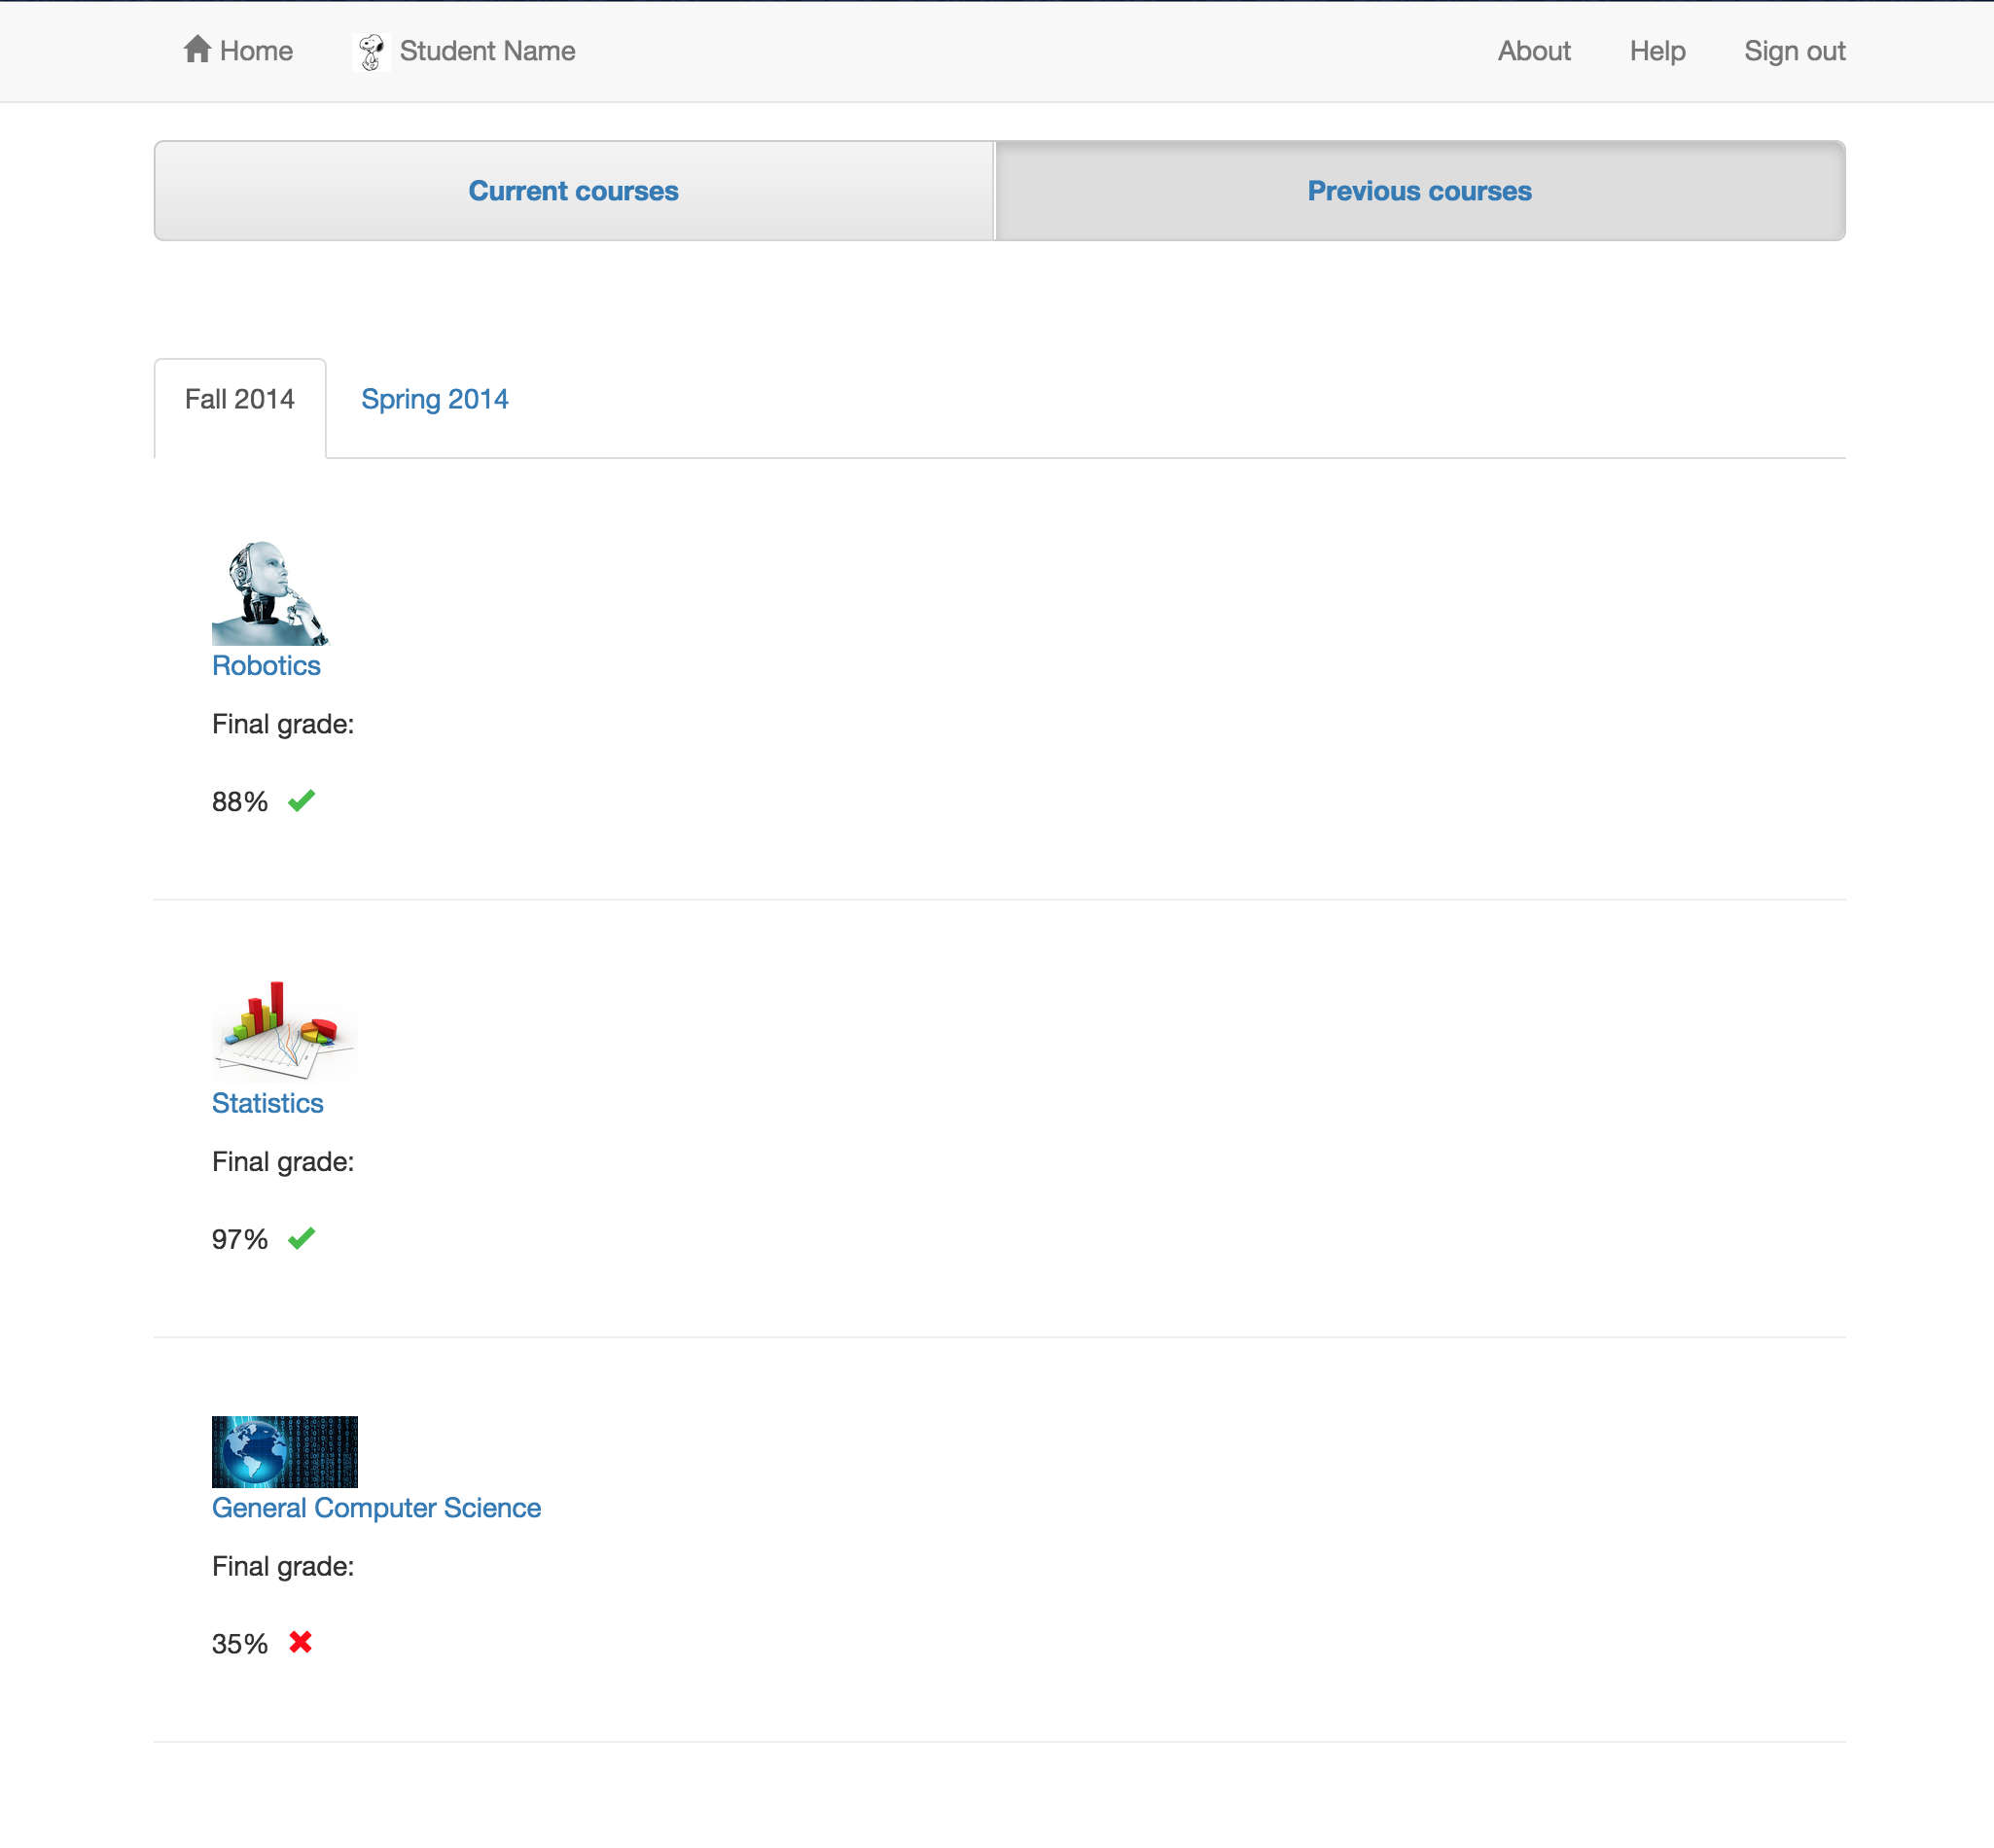
\includegraphics[width=\textwidth]{screenshots/PreviousCourses.png}

The current courses page features a sparse, left-justified layout in order to simplify the task of getting to the course page the user needs--minimal information beyond a grade overview, large \& attention-catching course icons, and the page navigation buttons is included. Following the rule-of-thirds by left-justifying the content helps the user process the information quicker.
